\chapter{Developer documentation}
\label{ch:impl}

This chapter gives the very details of involved technologies, development environment, analysis, implementations and considerations.

\section{Environment Requirements}
The application is supported to be ran and developed both locally and with dedicated cloud application: 
\begin{enumerate}
    \item Possible toolkit for Local environment
        \begin{itemize}
            \item Eclipse with Spring Tools and CAP extensions
            \item Visual Studio Code with SAP CAP extensions
            \item Intellij with SAP CAP extensions (recommanded for java development)
        \end{itemize}
    \item Possible toolkit for Cloud environment
        \begin{itemize}
            \item SAP Business Application Studio with Full-Stack Development dev-space (recommanded, used in this thesis)
        \end{itemize}
\end{enumerate}

For local development, up to date Java JDK, node.js and CAP extensions are hard requirements. The specific set up can be find \hyperlink{https://developers.sap.com/tutorials/btp-app-prepare-dev-environment-cap.html}{here}.

This thesis used SAP Business Application Studio (BAS) as development tool, which is ready for use. 

A snapshot of versions at the time of development:

\lstset{caption={Version check}, label=src:1}
\begin{lstlisting}[language={bash}]
> java --version
# openjdk 17.0.4.1 2022-08-12 LTS
# OpenJDK Runtime Environment SapMachine (build 17.0.4.1+1-LTS)
# OpenJDK 64-Bit Server VM SapMachine (build 17.0.4.1+1-LTS, mixed mode, sharing)
> cds version
# @sap/cds: 7.2.1
# @sap/cds-compiler: 4.0.2
# @sap/cds-dk: 7.2.0
# @sap/cds-dk (global): 7.2.0
# @sap/cds-fiori: 1.1.0
# @sap/cds-foss: 4.0.2
# @sap/cds-mtxs: 1.11.0
# @sap/eslint-plugin-cds: 2.6.3
# Node.js: v18.14.2

\end{lstlisting}


\section{Run}
The following commands can be used to run the application for testing.

\lstset{caption={Run commands}, label=src:22}
\begin{lstlisting}[language={bash}]
cds watch # The quickest way to check the exposed services on a browser.
\end{lstlisting}

If custom Java code is added, use the following command to run the services as a spring-boot application.
\begin{lstlisting}[language={bash}]
mvn clean install # This will compile *.cds files and create gen folder.
mvn spring-boot:run # THis will start the server at port 8084
\end{lstlisting}


\section{Analysis and Design}

This chapter explains the reason of the need of this application and lists the analysed necessary capabilities of the developed application.

\subsection{Business Context}
The application is aimed to provide an end to end streamlined procedure from the moment a parcel arrived at the reception to the second user confirm the pickup (package management). It also provides humane functions to ease the management of any parcel related information (storage and delivery companies management).

These are detailed in the following sub-sections. For each management requirement, user stories and user diagrams are given.

\subsection{Package Management}
Package management is the most the and center function of the application. It is responsible for register a parcel, confirm a parcel, pickup a parcel and review the history of the parcel.

\subsubsection{User Stories}
\subsubsection{User Diagram}

\subsection{Storage Management}

\subsubsection{User Stories}

\begin{table}[h]
\centering
\begin{tabular}{|p{2cm}|p{2.7cm}|p{2.7cm}|p{2.7cm}|p{2.7cm}|}
\hline
\textbf{As a} & \textbf{I Want To} & \textbf{Given} & \textbf{When} & \textbf{Then}\\
\hline
Player & Build a Road & I am in Road Construction mode. & I click on an empty general zone. & The program adds the road to the clicked zone. \\
\hline
Player & Build a Road & I am in Road Construction mode. & I click on a non-empty zone of any type & The program warns the player not able to build the road. \\
\hline
\end{tabular}
\caption{User Stories}
\end{table}

\subsubsection{User Diagram}

\subsection{Companies Management}
\subsubsection{User Stories}

\subsubsection{User Diagram}

% -----------------------------------------------
% Application Structure


\section{Application Structure}

The application is developed under the guidence of CAP (Cloud Application Programming Model) which is heavily based on CDS (Central Domain Service). Generally speaking, it contains one Java Spring-boot application as back-end and 7 Fiori UI applications dedicated to the 7 provided services. The communication between front-end and back-end is ensured under OData protocol over HTTPs. CDS views are used for data modelling and CDS annotations are used for service related definition and UI implementations.

\subsection{App structure}

The overall view of the application is the following:

\begin{figure}[H]
	\centering
	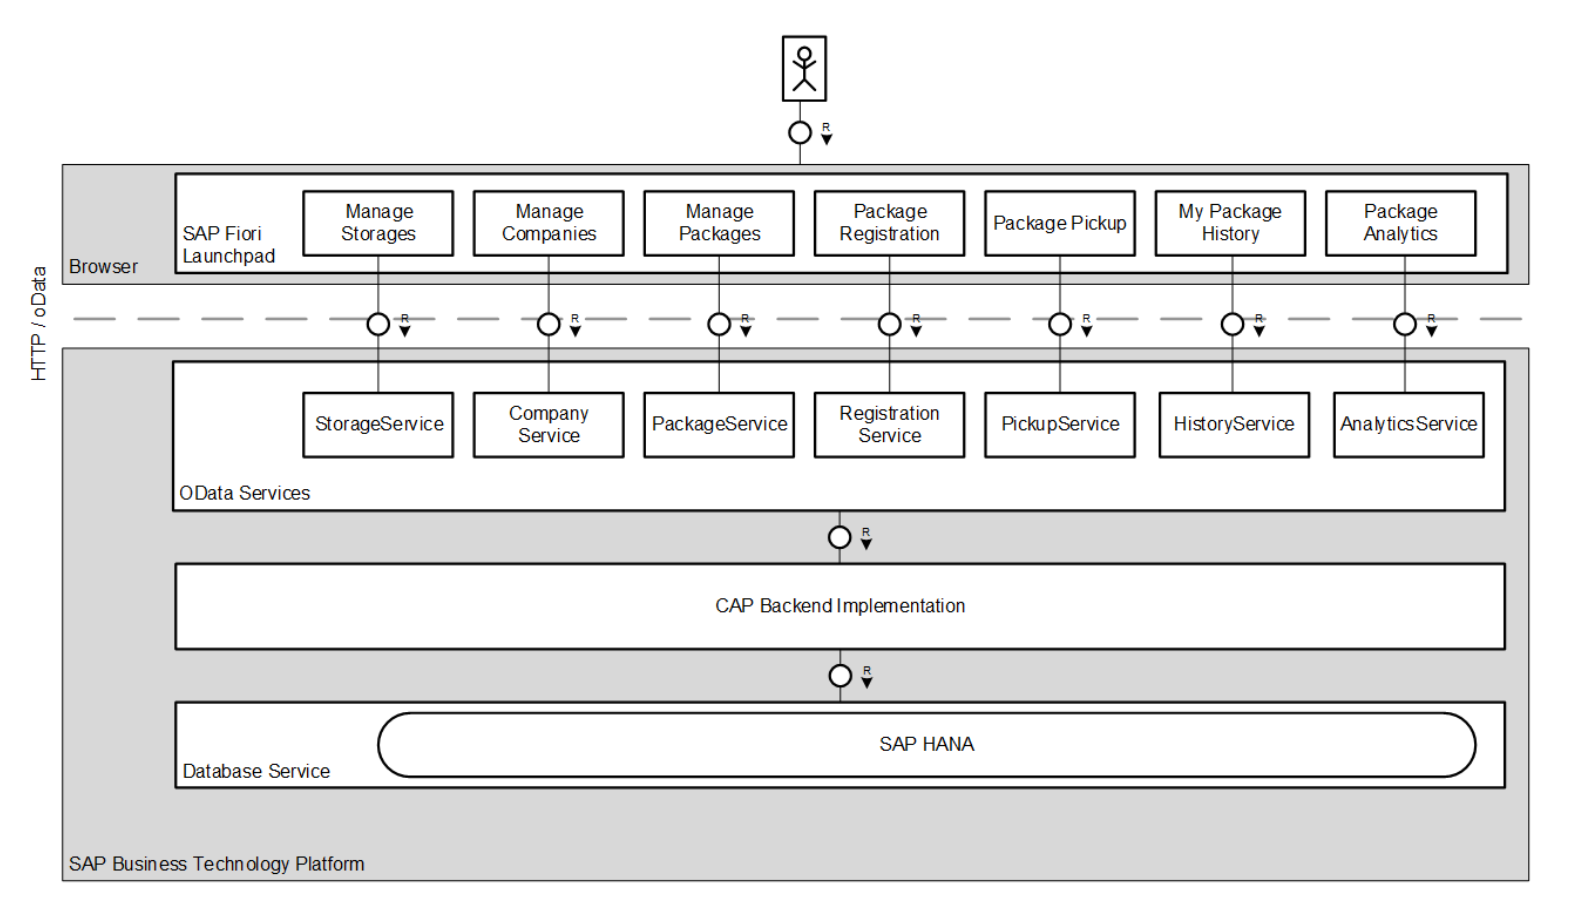
\includegraphics[height=250px]{images/Application_Structure.png}
	\caption{Application Structure Overview}
	\label{fig:appStruct}
\end{figure}

\subsection{Development Component}

All three essential parts of the application, front-end, back-end and database model are being developed at the same place/project/root directory. The implementations and definitions located in different directories of the project are logically packaged into seperate namespaces (namespace in CDS, package declaration in Java), as shown following:

\begin{figure}[H]
	\centering
	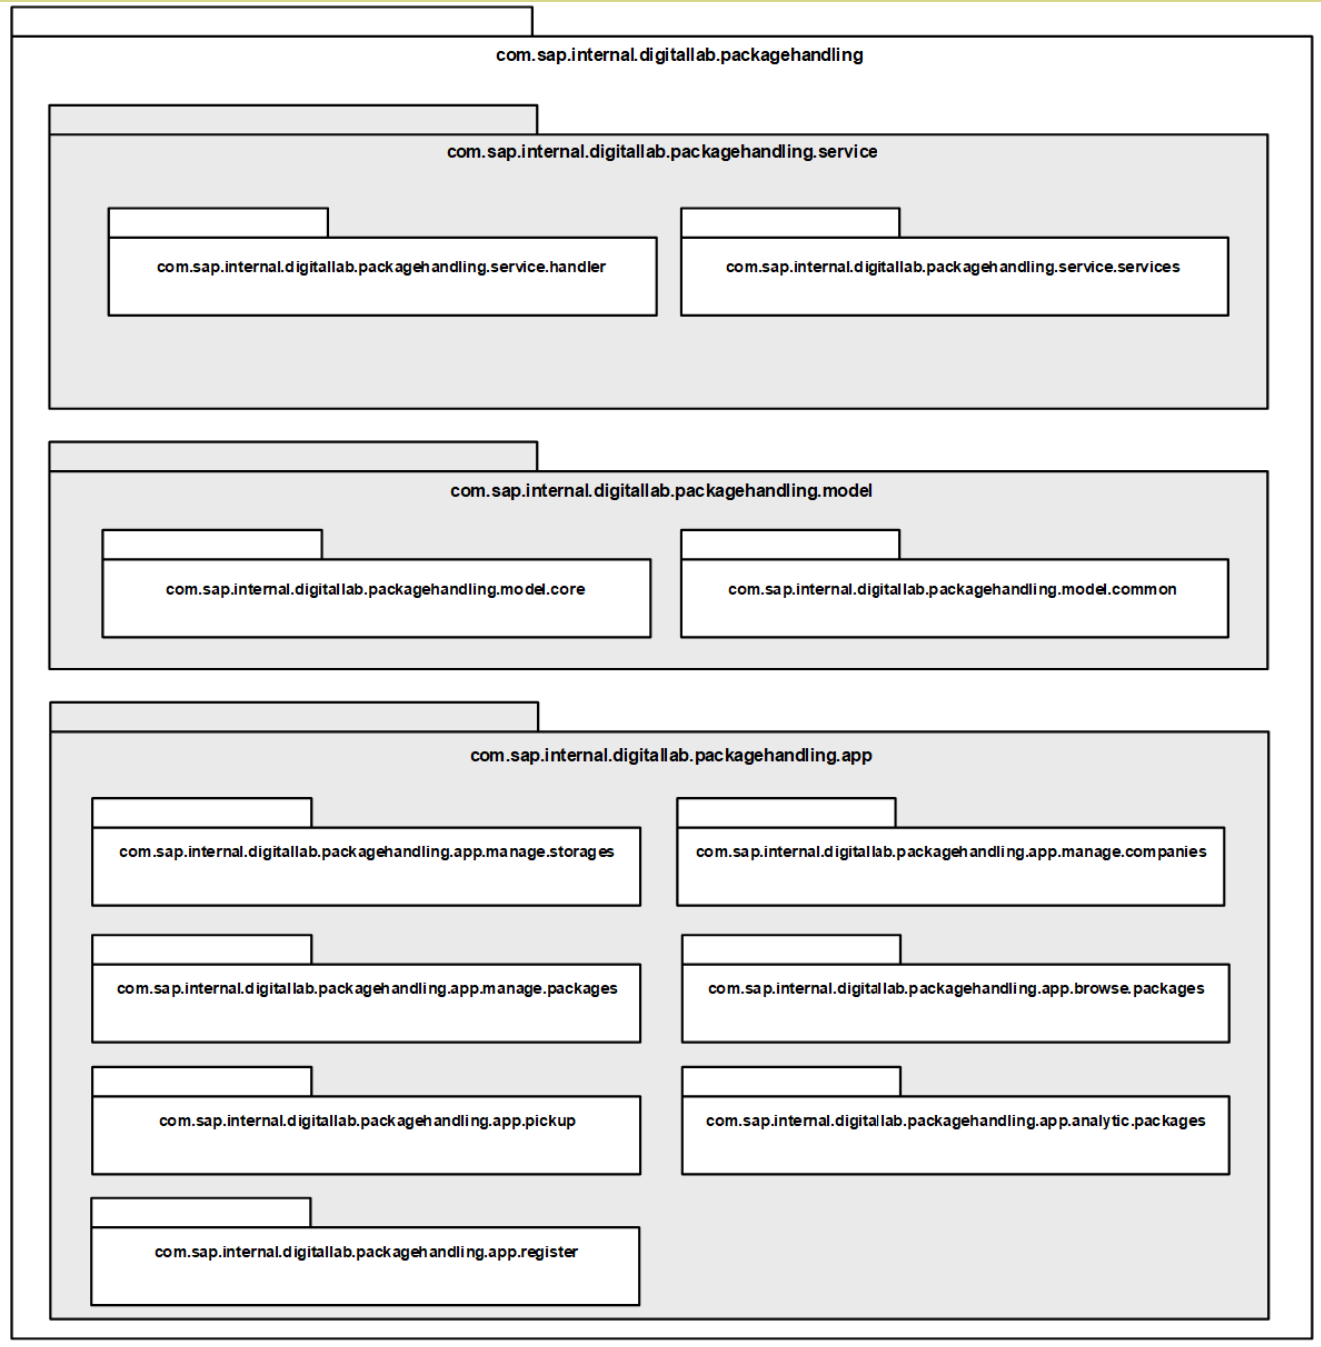
\includegraphics[height=400px]{images/Package_Diagram.png}
	\caption{Namespace Diagram}
	\label{fig:packStruc}
\end{figure}


\subsection{Project Structure}

The general directory structure of the application, which is a default CAP project set-up, can be peeked as the following:

\lstset{caption={Base project folders}, label=src:3}
\begin{lstlisting}[language={bash}]
root/
    |- srv # contains back-end service related implementations
    |- db # contains data model definitions and initial data
    |- app # contains all Fiori front-end applications
\end{lstlisting}

The details of inner parts of each directory will be introduced later in corresponding sections.

\section{Data Model}
Since Digital Lab provides more then one solutions and to ensure the maximum reuse of models, data model is seperated into 2 parts: solution specific data models and common data models, where the common data models are implemented separately of their own services. At the development time of this application, the common data service is not constructed yet, so they are implemented as part of the application as a PoC.

\subsection{ER Digram}
\subsubsection{Solution specific data model}

Here is a ER diagram of the solution specific data model.
picture
\subsubsection{General common data model}

Here is a ER diagram of the common data model.
picture

\subsection{Implementation}
All data models are modeled by CDS' definition language as a CDS view. Single entities are put into their own \textit{EntityName.cds} files. The main goal is to model out the exact relationships as illustrate in the specification section.

Here list the structure of folders:
\lstset{caption={Structure of folders - data model}, label=src:4}
\begin{lstlisting}[language={bash}]
root/
    |- db/
        |- data
        |- model
            |- packagehandling 
                |- *.cds # Definition of solution specific data model
            |- common
                |- *.cds # Definition of common data model
\end{lstlisting}

The correctness of the relationship implementation can be checked by running a command:

\lstset{caption={Generate schema from CDS view}, label=src:bash}
\begin{lstlisting}[language={bash}]
> cds compile ./db/models/common/ --to sql > schema.sql
\end{lstlisting}

In the root directory, one can find \textit{schema.sql} which will contains the DDLs of generated tables in HANA SQL.

The namespaces (as mentioned in application structure section) of the solution-specific and common data models are defined accordingly at the top of each entity definition.

\lstset{caption={cds namespaces for data model}, label=src:6}
\begin{lstlisting}[language={c++}]
// namespace for reused
namespace com.sap.internal.digitallab.packagehandling.common; 
// namespace for solution-specific
namespace com.sap.internal.digitallab.packagehandling.core; 
\end{lstlisting}


To optimize and standardize the outcome, common \textbf{aspects} (\textit{cuid, managed, User, CodeList}) from \textit{@sap/cds/common} are used in the definition. It can be seen as "extend" in the object-orient way, or more speificly "interface" in Java. Aspects are defined in a similiar way as entities, consists of fields/properties. Entities can "implement" zero to more aspects, "inheriting" aspect's properties and "extend" with its own properties. 

\begin{definition}
    \textbf{CDS's aspects} allow to flexibly extend definitions by new elements as well as overriding properties and annotations. They're based on a mixin approach as known from Aspect-oriented Programming methods.
\end{definition}

Here records the common aspects used by this thesis. \textit{managed} comes with 4 elements: created, created, changed, changed, and automatically updates them. \textit{cuid} automatically assigns UUID primary key to entity. \textit{CodeList} provides a out of box way of implementing enumeration like data structures and supports automatic localization.

\lstset{caption={Aspect managed from @sap/cds/common}, label=src:7}
\begin{lstlisting}[language={c++}]
aspect managed {
  createdAt  : Timestamp @cds.on.insert : $now;
  createdBy  : User      @cds.on.insert : $user;
  modifiedAt : Timestamp @cds.on.insert : $now  @cds.on.update : $now;
  modifiedBy : User      @cds.on.insert : $user @cds.on.update : $user;
}
\end{lstlisting}

\lstset{caption={Aspect cuid from @sap/cds/common}, label=src:8}
\begin{lstlisting}[language={c++}]
aspect cuid {
  key ID : UUID; //> automatically filled in
}
\end{lstlisting}

\lstset{caption={Aspect CodeList from @sap/cds/common}, label=src:9}
\begin{lstlisting}[language={c++}]
aspect CodeList @(
    cds.autoexpose,
    cds.persistence.skip : 'if-unused'
) {
    name  : localized String(255)  @title : '{i18n>Name}';
    descr : localized String(1000) @title : '{i18n>Description}';
}
\end{lstlisting}

Unique constraints are modeled with \textit{@assert.unique.<constraintName>} annotations at model level, enforcing uniqueness checks on all possible CREATE and UPDATE operations.

Below captures two examples from the thesis on usage of aspects coupled with the SQL DDL corresponding to the cds definition.
\lstset{caption={managed, cuid delivery company entity with unique constraint and corresponding SQL DDL}, label=src:10}
\begin{lstlisting}[language={sql}]
@assert.unique: {nbunique: [name]}
entity DeliveryCompany : cuid, managed {
    name     : String(255) not null;
    logo     : String(255)  @Core.IsURL  @Core.IsMediaType;
    packages : Association to many Package
                   on packages.deliveryCompany = $self;
}

CREATE TABLE com_sap_internal_digitallab_packagehandling_core_DeliveryCompany (
  ID NVARCHAR(36) NOT NULL,
  createdAt TIMESTAMP(7),
  createdBy NVARCHAR(255),
  modifiedAt TIMESTAMP(7),
  modifiedBy NVARCHAR(255),
  name NVARCHAR(255) NOT NULL,
  logo NVARCHAR(255),
  PRIMARY KEY(ID),
  CONSTRAINT core_DeliveryCompany_nbunique UNIQUE (name)
); 
\end{lstlisting}

\lstset{caption={codelist package type entity and corresponding SQL DDL}, label=src:11}
\begin{lstlisting}[language={sql}]
entity PackageType : sap.common.CodeList {
    key code : String(255) not null;
}

CREATE TABLE com_sap_internal_digitallab_packagehandling_core_PackageType (
  name NVARCHAR(255),
  descr NVARCHAR(1000),
  code NVARCHAR(255) NOT NULL,
  PRIMARY KEY(code)
);
\end{lstlisting}
\section{Security}
The application is defined and developed for internal use of company, that is, can be accessed only from SAP devices. The application uses XSA Security and Authentication Service (XSUAA) as for Authentication. Authorization of the application is enforced through a role based accessibility to the specific services. Four roles are defined, namely Administrator, Facility Manager, Receptionist and End-User. The assignment of roles is done centrally on the Business Technology Platform (BTP), some mock users are also defined for the local development environment.


\subsection{Roles Specification}
All role-specific are set up in the file \textit{root/xs-security.json}. The according restriction on services are defined in \textit{root/srv/services/*-auth.cds} files. As illustrated below.

\lstset{caption={File locations - Security}, label=src:12}
\begin{lstlisting}[language={bash}]
root/
    |- srv/
        |- src
        |- gen
        |- services
            |- ServiceName 
                |- *.cds # Definition of service
                |- *-auth.cds # Access restriction on roles.
    |- xs-security.json # list of roles
\end{lstlisting}

The access rules of the 4 roles are listed below:

\begin{table}[H]
    \centering
    \begin{tabular}{|c|c|c|c|c|} \hline 
         &  End-User&  Facility Manager&  Administrator&  Receptionist \\ \hline 
         Manage Storage& No  & Yes & Yes & No  \\ \hline 
         Manage Delivery Companies& No & Yes & Yes & No  \\ \hline 
         Manage Packages& No & Yes & Yes & Yes \\ \hline 
         Package Pickup& Yes & Yes & Yes & Yes  \\ \hline 
         Package Registration& No & Yes & Yes & Yes \\ \hline 
         My History& No & Yes & Yes & No \\ \hline
    \end{tabular}
    \caption{Roles Access Rules}
    \label{tab:Access Rule}
\end{table}

\subsection{Mock Users}
To support local development and testing, 4 mock users are defined under \textit{application.yaml}, which will be used in the default spring boot run-time.

Here pasted an example of mock user.

\lstset{caption={Mock Users - Security}, label=src:yaml}
\begin{lstlisting}[language={bash}]
security:
    authentication.normalize-provider-tenant: true
    mock.users:
        admin:
            password: admin
            roles:  
                - Administrator 
        user:
            password: user
                - User
        manager:
            password: manager
            roles:
                - FacilityManager
\end{lstlisting}

\section{UI}
<<Introduce UI5>>
The application utilized UI5 Fiori elements. Every UI related modules are packed under \textit{root/app} folder and then into its dedicate \textit{servicename-ui} folder. In short, Fiori elements are assembled into pages using cds annotations on the exposed services. App router is added to direct urls throughout backend OData services and frontend Fiori web application and \textit{appconfig} compiles the used UIs onto Fiori Launchpad. End-points are defined again inside \textit{application.yaml}.

\subsection{Front-end Architecture Overview}

\subsubsection{Things to Do}

The main way to add a UI for a service is to create a standard-alone UI5 application using the dedicate service under the app folder, customize the UI with annotations and register it inside appconfig.

With the annotations, the type of components (lists, object, etc.) is defined for each entities exposed by certain service in the places (header, body, footer).

\subsubsection{File Structure}
\lstset{caption={File locations - UI}, label=src:14}
\begin{lstlisting}[language={bash}]
root/
    |- app/
        |- servicename-ui
            |- webapp
            |- annotation.cds # Custom UI for entities exposed by the service.
        |- appconfig # UIs' config for Fiori Launchpad sandbox.
        |- router
        |- fiori.html # welcome page for app router.
        |- index.html # welcome page in case of backend start by maven.
\end{lstlisting}

\subsection{Manage Storage}
\subsubsection{Manifest}
\subsubsection{Components}

\subsection{Manage Company}
\subsubsection{Manifest}
\subsubsection{Components}

\subsection{Manage Package}
\subsubsection{Manifest}
\subsubsection{Components}

\subsection{Register Package}
\subsubsection{Manifest}
\subsubsection{Components}

\subsection{Pickup Package}
\subsubsection{Manifest}
\subsubsection{Components}

\subsection{My Package}
\subsubsection{Manifest}
\subsubsection{Components}


\section{Services}

As mentioned in the above sections, 6 OData end-points are maintain by the back-end. This section will first give an general overview of the folders, packages, steps of implementing a service, which are shared by every provided service, then will give more detailed and specific information on each of the service.

\subsection{Back-end Architecture Overview}

\subsubsection{Things to Do}

The implementation of back-end services are done using a combination of two languages: CDL (CDS' definition language) and Java.

\bigskip
The first step of implementing any service is to define its CDS view using CDL, which provides instructions on:
\begin{compactenum}
	\item The data model in database to be exposed by the service.
	\item The desired input validations.
	\item The capabilites of action controls.
    \item The role restrictions on the access of the application.
    \item (Optional) actions and functions dedicated to the service.
\end{compactenum}

\bigskip

The second step is implementing the business logic using Java. CAP project provides a out-of-box default implementation of simple CRUD operations, in some cases shall be override/replaced. In most of the cases it involves explicit interactions with the persistence service and in this case a Java supported CQN (Core Query Notation) is used. The Java codes should applies the following:
\begin{compactenum}
	\item Implementations of custom CRUD operations
	\item Implementations of virtual fields calculations
	\item Implementations of actions and functions defined in CDS view.
\end{compactenum}

\subsubsection{Pre-knowledge}
To fully understand how to write these implementation, one should first recognize the \textit{srv/gen} folder, which contains generated Java codes by cds builder. Here lists the very necessary pre-knowledges and factors on the generate code, before continuing with implementations. 
\begin{compactenum}
	\item \textit{srv/gen} folder is generated from all the \textit{*.cds} files using in the \textit{index.cds} (recursively used), for an entity or a service definition.
    \item The generated code are in Java and are under the same package domain as specified in namespace of the \textit{*.cds} files.
    \item For each entity and service a couple of \textit{EntityName.java} and \textit{EntityName\_.java} interface being generated. 
    \item One can use \textit{EntityName\_.CDS\_NAME} in case of the need to clarify the usage of certain entity or service. Also \textit{EntityName\_.class} in CQN as an analogy of table names. 
    \item One shall use \textit{EntityName} in case of the usage of the real entity or service, similiar to object model in JPA. Also in the case of CQN, constants of column names can be retrieved as static fields like this: \textit{EntityName.COLUMN\_NAME}, which should be encouraged over giving string expressions.
\end{compactenum}

\bigskip
It is also important to understand the event processing of CAP. CAP provides out of box handling of CRUD event for every entity and the costume logics are implemented using the idea: what should happen before, on and after the event, with the help of method annotation \textbf{@Before, @On, @After}. Methods annotated with \textbf{@Before} and \textbf{@After}, as the name suggested, implements preprocessing and postprocessing logic. \textbf{@On} can be seen as an override of the origin defalut implementation of the event. For a custom event or action, it is obligaory to provide an \textbf{@On} method.

\subsubsection{Architecture Design}

The back-end architecture follows the recommendations of CAP, Spring MVC and microservices architecture principles. Its implementation is divided into 3 layers: handlers, managers and repositories. Upon a OData service request, queries are forwarded to the so called Consumption API which then triggers the generic event handlers of CAP passing a so called event context. At this point, handler layers came into play and dispatch the tasks associated with the event to manager layers, where business logics (processing/caculations) are coded. In case of a interaction with database models, the processing is delegated to the repository layer, which implements sets of database related operations at Java level using CQL (CDS Query Language) communicating with CQN execution engine. 

\subsubsection{Layers in Details}

\begin{figure}[H]
	\centering
	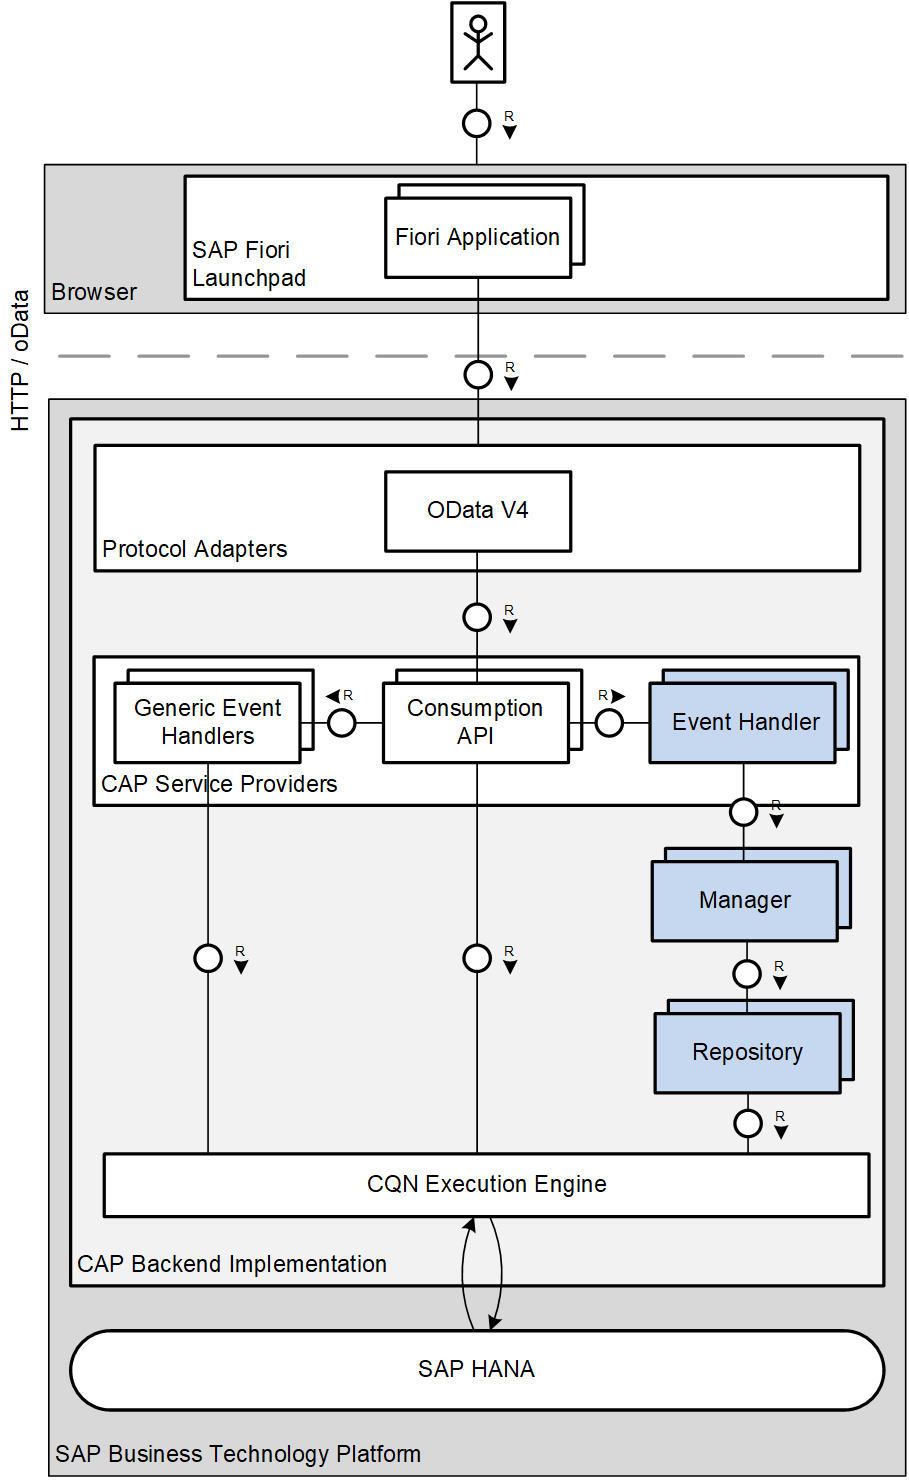
\includegraphics[height=400px]{images/backend_architecture.png}
	\caption{Back-end architecture}
	\label{fig:backArch}
\end{figure}

The blocks in blue of the above figure indicates the necessary Java implementation parts. In the handler layer, a \textit{<ServiceName>ServiceHandler} class is defined for every service and each handler implements the \textbf{EventHandler} from cds's came along package \textit{com.sap.cds.services.handler}. This ensures that the handler class will be fed with received events from the Consuming API. Also a Java annotation \textbf{@ServiceName(SomeService\_.CDS\_NAME)} is added at class level, to provide information on which service the handler is handling. The handlers classes are also marked with \textbf{@Component} annotation from the spring framework as a Bean, to get the most out of Spring-boot's dependency control. A base skeleton of handler class is embedded below:

\lstset{caption={Handler skeleton - Backend}, label=src:2008}
\begin{lstlisting}[language={java}]
@Component
@ServiceName(EnvolvedService_.CDS_NAME)
public class EnvolvedServiceHandler implements EventHandler { }
\end{lstlisting}

In case of necessary usage of manager layer, private field and auto-wired constructor injection combination is used, as supported by the spring-boot framework. A base skeleton of class association (composition in spring-boot implementation aspect) below:

\lstset{caption={Association class skeleton - Backend}, label=src:2018}
\begin{lstlisting}[language={java}]
private final UsedEntityManager manager;

@Autowired
public CompanyServiceHandler(UsedEntityManager manager) {
    this.manager = manager;
}
\end{lstlisting}

To explicitly watch an event (CRUD, custom events/actions/functions), methods should look like this:
\lstset{caption={Listening method skeleton - Backend}, label=src:2019}
\begin{lstlisting}[language={java}]
@After(event = {CqnService.EVENT_DELETE})
public void afterDeleteEvent(EventContext context) { }
\end{lstlisting}

\bigskip
**Note: The complete reference of supported annotations and arguments types can be find inside the CDS documentation, and would not be detailed in this thesis. Only syntax essential for reading the thesis codes are explained.

\bigskip
In the manager layer, a \textit{<EntityName>Manager} class is defined for every entities. Each class contains entity related methods to support the services. It holds every required calculations, processing, business logics partitioned by entities. It can be more or less analog to the service layer in a normal back-end spring-boot application.

A base skeleton of manager class would be something like the following:

 \lstset{caption={Manager class skeleton - Backend}, label=src:3000}
\begin{lstlisting}[language={java}]
@Component
public class OneEntityManager {
    private final OneEntityRepository repo1;
    private final OneOtherEntityRepository repo2;
    private final OtherEntityManager mgr;
    ...

    @Autowired
    public PackageManager(OneEntityRepository repo1, OneOtherEntityRepository repo2, OtherEntityManager mgr) {
        this.repo1 = repo1;
        this.repo2 = repo2;
        this.mgr = mgr;
    }

    public void someMethodHandlingTheRequestsFromHandlerClass() {}
    private void someHelperMethod() {}
}
\end{lstlisting}


\bigskip
In the repository layer, a \textit{<EntityName>Repository} class is defined for every entities. This layer can be seen as the model layer in MVC architecture. It is responsible for any direct interaction with the database. In CAP, the connection to database is provided through a persistence service implementation (\textbf{com.sap.cds.services.persistence.PersistenceService}) so that different databases (sqlite at development environment, HANA at deployment) can be used and switched seamless. CQN builders are also provided under \textbf{com.sap.cds.ql.cqn} supporting a SQL like syntax for building a SQL statement in Java.

 A base skeleton of repository class is shown below:

 \lstset{caption={Repository class skeleton - Backend}, label=src:3000}
\begin{lstlisting}[language={java}]
@Component
public class DeliveryCompanyRepository {
    private final PersistenceService db;

    @Autowired
    public DeliveryCompanyRepository(PersistenceService db) {
        this.db = db;
    }
}
\end{lstlisting}

To interacted with the database, a CQN example is provided here:

 \lstset{caption={CQN method skeleton - Backend}, label=src:3001}
\begin{lstlisting}[language={java}]
/**
 * SELECT * FROM delivery_company WHERE id = $id;
 *
 * @param id company UUID to check.
 * @return resulting rows
 */
public Result selectById(String id) {
    CqnSelect select = Select
            .from(DeliveryCompany_.class)
            .byId(id);
    return db.run(select);
}
\end{lstlisting}

\subsubsection{Debug}

To support debugging, a \textbf{Logger} is added to every class to provide logging statements.

\lstset{caption={Logger - Backend}, label=src:2009}
\begin{lstlisting}[language={java}]
 private static final Logger LOGGER = LoggerFactory.getLogger("name_logger");
\end{lstlisting}


\subsubsection{File structure}
Below one can also find an illustration of the real folder structures.

\lstset{caption={Directories guide - Back-end}, label=src:15}
\begin{lstlisting}[language={bash}]
root/
    |- srv/
        |- src # Java codes for custom business logics
            |- main/java/com/sap/internal/digitallab/
                |- packagehandling
                    |- handlers
                        |- <ServiceName>Handler.java
                    |- managers
                        |- <EntityName>Manager.java
                    |- repositories
                        |- <EntityName>Repository.java
        |- gen # generated java codes from CDS views
        |- services # Service definitions in CDS annotation
            |- ServiceName 
                |- *.cds # otehr definition of service
                |- *-auth.cds # Access restriction on roles.
\end{lstlisting}

\subsection{Storage Service}
Storage service serves the purpose of holding information on the possible storage places and keep track of the usages of single storage slots with the storage. Entities being exposed by the service are:

\subsubsection{Details}

\begin{compactenum}
	\item Storage (*)
    \item StorageSlot (*)
    \item Building (id, name, map, address, coordinates, phoneNumber)
    \item BuidingFloor (id, name, map, building)
    \item SlotStatus (*)
\end{compactenum}

\bigskip
In the service's CDS view, input invalidation checks are also defined for mandatory fields using \textbf{@mandatory} annotation. This ensures the rejection of creation in case of missing fields. \textbf{@read-only} annotation is used to insure the non-editable fields and association (foreign key validation) is reinforced by \textbf{@assert.target}, which will check the existence of the foreign key at runtime.

\bigskip
Mandatory fields of storage service:
\begin{compactenum}
	\item Storage.name
    \item Storage.buildingFloor
    \item StorageSlot.name
    \item StorageSlot.storage
\end{compactenum}

\bigskip
Read only fields of storage service:
\begin{compactenum}
	\item StorageSlot.status
\end{compactenum}

\bigskip
Reinforced foreign keys of storage service:
\begin{compactenum}
	\item StorageSlot.storage
\end{compactenum}

\bigskip
**Note: Storage.buildingFloor is not checked as a foreign key here, because in the plan its reference should be replaced by a central data service.


A custom action \textit{massCreate} is implemented, which creates multiple slots at one shot. The implementation also watches the read events of \textbf{Storage} and \textbf{StorageSlot}, after which virtual fields (\textit{total packages}, \textit{current packages}) and virtual action control fields (\textit{delete ac}) are calculated dynamically.

\subsubsection{UML}

Classes and methods related to storage service is illustrated in the UML. Private utility methods are ignored for the sake of simplicity.
\begin{figure}[!h]
    \centering
    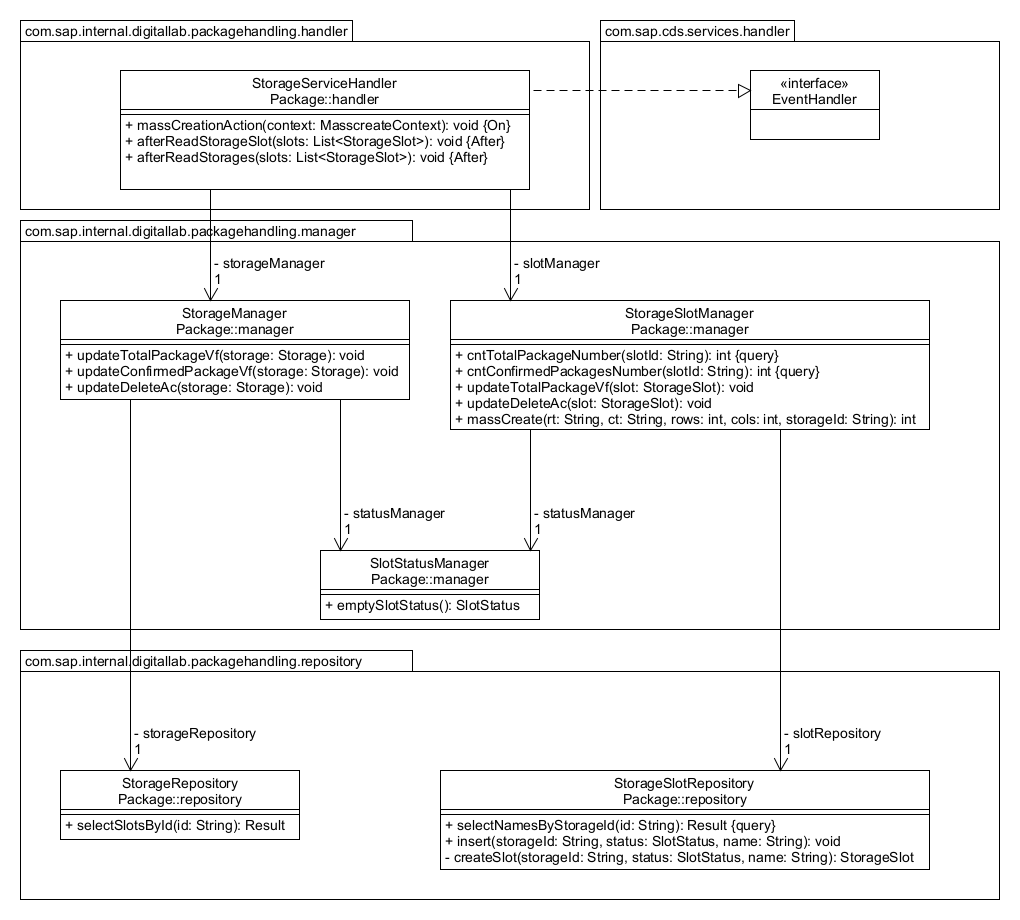
\includegraphics[width=1\linewidth]{images/service_class_diagrams/storage_service_class_diagram.png}
    \caption{Storage Service UML}
    \label{fig:storage_service_uml}
\end{figure}
\pagebreak

\subsection{Company Service}
Company service provides the possibilities for facaulty managers and administrators to CRUD the delivery companies and is exposed under the end-point \textbf{api/CompanySerive}.

\subsubsection{Details}

Enities being exposed by the service are:
\begin{compactenum}
	\item DeliveryCompany (*)
\end{compactenum}

\bigskip
In the service's CDS view, input invalidation checks are also defined for mandatory fields using \textbf{@mandatory} annotation. This ensures the rejection of creation in case of missing fields. 

\bigskip
Mandatory fields of storage service:
\begin{compactenum}
	\item DeliveryCompany.name
\end{compactenum}

\subsubsection{CRUD}
CRUD are supported for a delivery company entity. Custom Java code ensures the relevant packages' references to the company are deleted seamlessly upon the deletion of the company.

\subsubsection{UML}

Classes and methods related to storage service is illustrated in the UML. Private utility methods are ignored for the sake of simplicity.
\begin{figure}[!h]
    \centering
    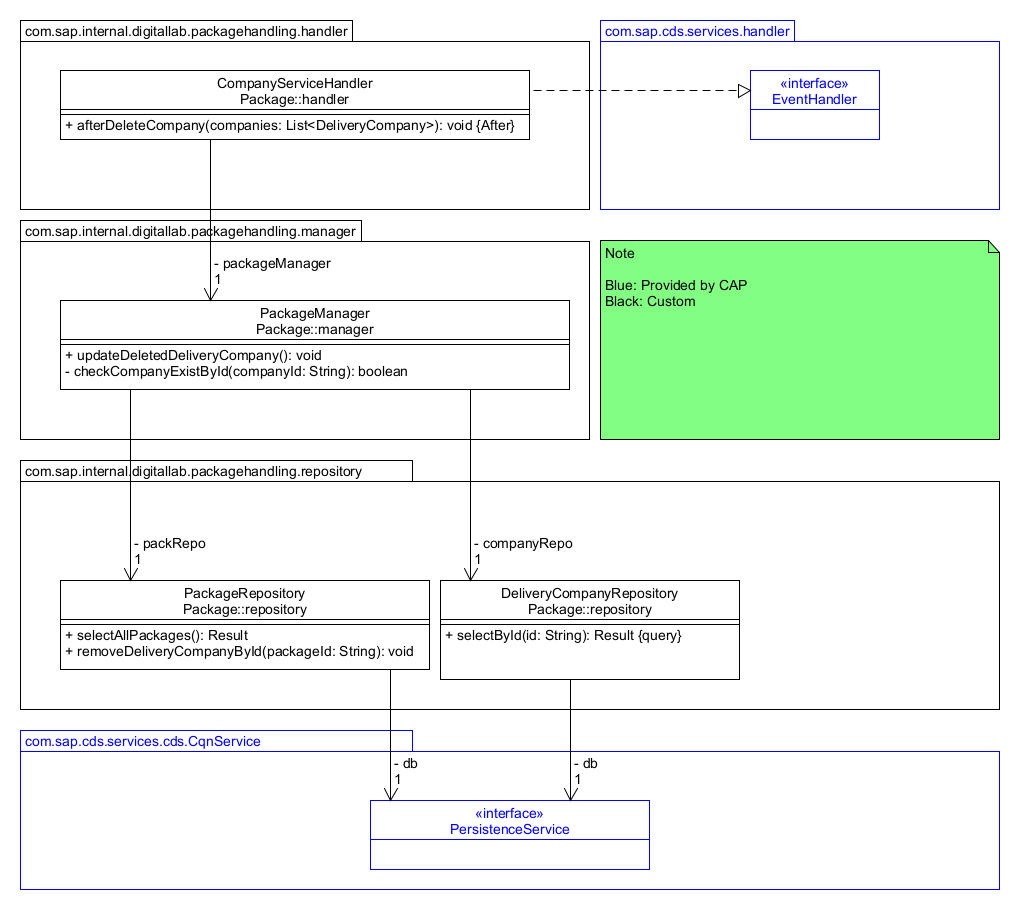
\includegraphics[width=1\linewidth]{images/service_class_diagrams/company_service_class_diagram.png}
    \caption{Company Service UML}
    \label{fig:company_service_uml}
\end{figure}
\pagebreak

% -------------------------------------
%  Package service
%  -----------------------------------
\subsection{Package Service}
Package service provides receptionists, faculty managers and administrators the abilities to update and delete a package and reads its related information. It is exposed at OData end-point \textit{api/PackageService} 

\subsubsection{Details}

Enities being exposed by the service are:
\begin{compactenum}
	\item Package (*)
    \item PackageType (*)
    \item PackageStatus (*)
    \item Storage (id, name, buildingFloor)
    \item StorageSlot (id, name, buildingFloor)
    \item DeliveryCompany (id, name, buildingFloor)
    \item Building (id, name, buildingFloor)
    \item BuildingFloor (id, name, buildingFloor)
\end{compactenum}

\bigskip
In the service's CDS view, input invalidation checks are defined for mandatory fields using \textbf{@mandatory} annotation. This ensures the rejection of creation in case of missing fields. \textbf{@read-only} annotation is used to insure the non-editable fields and association (foreign key validation) is reinforced by \textbf{@assert.target}, which will check the existence of the foreign key at runtime.

\bigskip
Mandatory fields of package service:
\begin{compactenum}
	\item Package.recipient
    \item Package.type
    \item Package.receptionist
\end{compactenum}

\bigskip
Read-only fields of package service:
\begin{compactenum}
	\item Package.recipient
\end{compactenum}

\bigskip
Reinforced foreign keys of package service:
\begin{compactenum}
	\item Package.type
\end{compactenum}

\bigskip
Two custom unbounded actions \textit{confirm} and \textit{pickup} are also defined in the CDS view, to facilitate the confirmation of a package (new -> confirmed) and the picked-up possibility of a package by a facility manager and administrator (confirmed -> pickup). Two action controls, \textit{confirm\_ac} and \textit{pickup\_ac} then are introduced coupling with the previous two actions, to make sure that the action button will only be available at desired time at the UI level. The bound is implemented with the \textit{@Capabilities} annotation. Furthermore, a delete action control is added on the package entity, which shall be activated only when a package is of status new / confirmed. This controls the activation of "delete" button at UI level specified by the \textit{@Capabilities} annotation. 

\bigskip
An useful detail here is that, the pickup action in the package service shall be used by receptionist and facility manager only, when the end-user cannot access to the pickup service (will be introduced later in the chapter). While both service have the same pickup action, the \textit{pickup\_ac} in package is shared by the two service.

\subsubsection{CRUD}
Read, update and delete possibilities of an package entity are guaranteed by the package service. For the other exposed entities, only read possibility is allowed. The reinforcement of CRUD capabilities can be checked in the \textbf{PackageService.cds}. 

\bigskip
An useful note here is that, the create operation of the package is missing in this service, as there is a seperated registration service which is only responsible for the creation of new package, which will be detailed later.

\subsubsection{UML}

The realization of the calculations of action control and the custom behaviour of actions are done in the Java part. The related slasses and methods can be checked in the UML. 

\begin{figure}[!h]
    \centering
    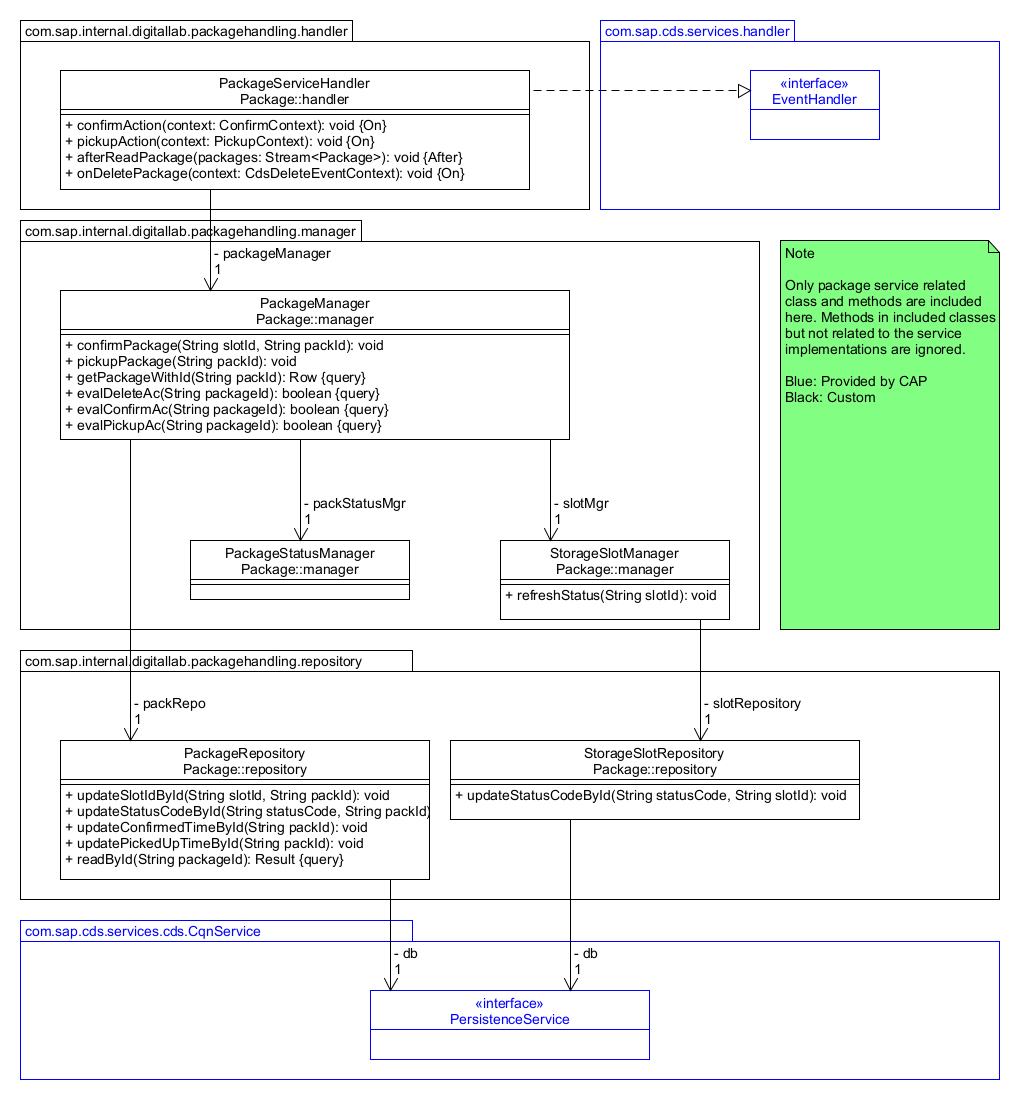
\includegraphics[width=1\linewidth]{images/service_class_diagrams/package_service_class_diagram.png}
    \caption{Package Service UML}
    \label{fig:package_service_uml}
\end{figure}
\pagebreak



% -------------------------------------
%  Registration service
%  -----------------------------------
\subsection{Registration Service}

Registration service provides receptionists, faculty managers and administrators the abilities to create (register) a package and reads its related information. It is exposed at OData end-point \textit{api/RegistrationService}. 

\bigskip
One thing to remember is that at this stage a package is only created but not stored, the status is all new and the storage details shall be determined in the previous package service. More details of the business logic can be check in the user documentation.

\subsubsection{Details}

Enities being exposed by the service are:
\begin{compactenum}
	\item Package (*)
    \item PackageType (*)
    \item PackageStatus (*)
    \item DeliveryCompany (id, name)
\end{compactenum}

\bigskip
In the service's CDS view, input invalidation checks are defined for mandatory fields using \textbf{@mandatory} annotation. This ensures the rejection of creation in case of missing fields. \textbf{@read-only} annotation is used to insure the non-editable fields and association (foreign key validation) is reinforced by \textbf{@assert.target}, which will check the existence of the foreign key at runtime.

\bigskip
Mandatory fields of package service:
\begin{compactenum}
	\item Package.recipient
    \item Package.type
    \item Package.receptionist
\end{compactenum}

\bigskip
Read-only fields of package service:
\begin{compactenum}
	\item Package.recipient
\end{compactenum}

\bigskip
Reinforced foreign keys of package service:
\begin{compactenum}
	\item Package.type
\end{compactenum}


\subsubsection{CRUD}
Create possibility of an package entity is guaranteed by the registration service. For the other exposed entities, only read possibility is allowed. The reinforcement of CRUD capabilities can be checked in the \textbf{RegistrationService.cds}. The reason behind these restrictions had already been discussed in the previous sector.

\subsubsection{UML}

This is a simpler service compare to the previous ones. No actions or action controls are defined for this service. Only a pre-processing (pre-fill the package status to new) is implemented at Java level and a simple handler class is pretty much all one would need. Nevertheless, the related classes and methods can be checked in the UML. 

\begin{figure}[!h]
    \centering
    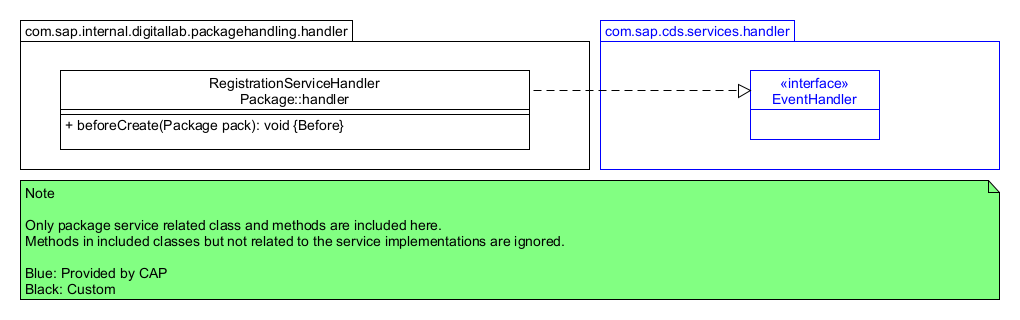
\includegraphics[width=1\linewidth]{images/service_class_diagrams/registration_service_class_diagram.png}
    \caption{Registration Service UML}
    \label{fig:registration_service_uml}
\end{figure}
\pagebreak




% -------------------------------------
%  Pickup service
%  -----------------------------------
\subsection{Pickup Service}

While the previous 4 services are doing uninteresting administration stuff and can be accessed only by nominated roles, here comes finally 2 service, opening to all end-users with a proper company device. One of them is the pickup service. As the name suggest, it provides any authenticated user the abilities to check and pickup his or her own confirmed package at the reception. It is exposed at OData end-point \textit{api/PickupService}. It is designed to be optimized for mobile use but this will be left to be discussed in the UI chapter.

\subsubsection{Details}

Entities being exposed in this service is almost the same as in the package service, with a little bit reduction, providing user with just enough necessary information. Entities exposed by the service are:
\begin{compactenum}
	\item Package (*)
    \item PackageType (*)
    \item PackageStatus (*)
    \item Storage (id, name, locationInstructions)
    \item StorageSlot (id, name)
    \item DeliveryCompany (id, name)
\end{compactenum}

\bigskip
In the service's CDS view, no input invalidation checks are defined, as the user will not be able to change anything, other than click a confirm pickup button. As for the future pickup button, an action \textit{pickup} is defined. Its entanglement with the \textit{pickup\_ac} used by package service are discussed in the previous sector.

\subsubsection{CRUD}
The same idea goes in the CRUD possibilities - only read operation is supported for any entity.

\subsubsection{UML}

A default filter read operation and the custom action are implemented in the Java part. The pickup action itself basically reuse the same methods as the package service does. The related classes and methods can be checked in the UML. 

\begin{figure}[!h]
    \centering
    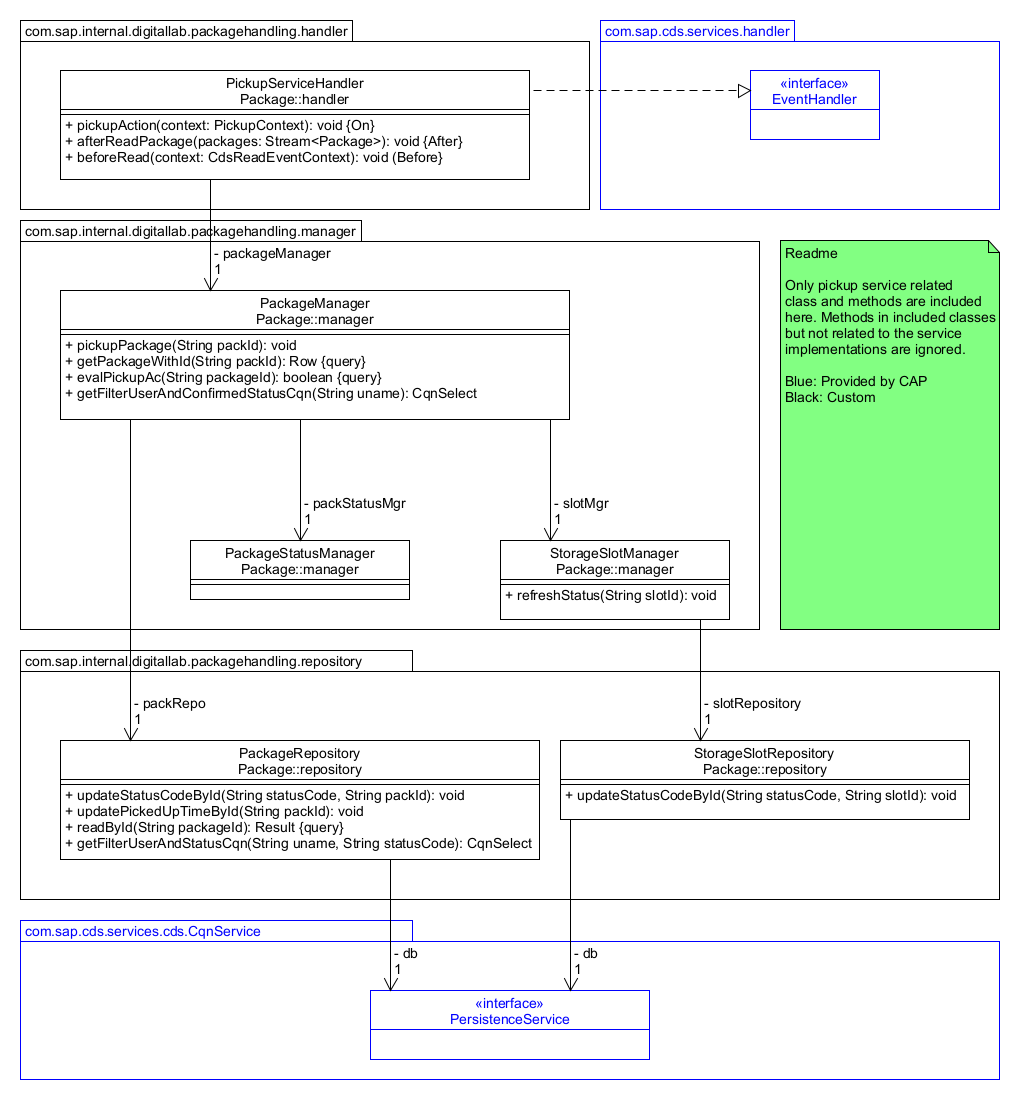
\includegraphics[width=1\linewidth]{images/service_class_diagrams/pickup_service_class_diagram.png}
    \caption{Pickup Service UML}
    \label{fig:pickup_service_uml}
\end{figure}
\pagebreak

% -------------------------------------
%  History service
%  -----------------------------------
\subsection{History Service}
History service serves for any authenticated user to check their package history.

\subsubsection{Details}

Entities being exposed in this service is almost the same as in the registration service, with every details, providing user with as much information as could. Entities exposed by the service are:
\begin{compactenum}
	\item Package (*)
    \item PackageType (*)
    \item PackageStatus (*)
    \item DeliveryCompany (*)
\end{compactenum}

\bigskip
In the service's CDS view, no input invalidation checks are defined, as the user will not be able to change anything. Nevertheless, a restriction makes user to only read about hos or her own package is defined with a \textit{where} statement in the projection view. Codes can be checked in \textit{HistoryService.cds} file.

\subsubsection{CRUD}
The same idea goes in the CRUD possibilities - only read operation is supported for any entity and this is enforced by a \textit{@readonly} annotation on every entity projection.

\subsubsection{UML}

There are no need of Java code to support the behaviour of the history service and hence no UML is included here.


\section{Testing}
The test strategy of this thesis is "test as it goes". Right after the implementation of services, unit tests on methods and integration tests on services are added. The same goes for UI implementation.

\subsection{Unit Testing}

\subsubsection{Implementation}
Unit testing focus on the methods and line coverage of the manager and the repository layer. JUnit 4 and spring test stater pack is used to write the tests. A test dedicated spring application environment is also defined in the \textit{application.yaml}. The main reason behind is that the initial data's loading path is different in the two environment.

\bigskip
A test class is created for each used class in the manager and repository layer. Those who are merely a placeholder for structure usages are ignored. Each test class is written under the following logic.

\begin{compactenum}
	\item An autowired instance of the class it is testing.
    \item 1..many test cases for each public method.
    \item Each test case calls a method and assert a desired output depends on the initial data in the csv files.
    \item Intellij coverage test is executed at the end of implementation to ensure every branch / edge cases are covered.
\end{compactenum}

\subsubsection{Extending Advice}
As stated in the above bullet points, the unit test depends largely on the existing test data. In case of any needs in the future that more test shall be added, it is advised to append completely new dedicated test data sets into csv. Delete or removing the existing data set can result in sever collapse of the current tests.

\subsection{Integration Testing}
Integration testing focus on the testing of back-end services, that is, on the handler layer. Rest Assure apit testing framework are used in couple with the spring's native api test SpringMockMvc.

Now I do not know how to use. TO BE CONTINUED>>>

\section{Deployment}

\section{Technologies and Terms}
